\documentclass[12pt]{article}
\usepackage{amsmath}
\usepackage{graphicx}
\usepackage{hyperref}
\usepackage[latin1]{inputenc}
\usepackage{listings}
\usepackage{pgfplots}
\renewcommand{\labelitemi}{$\textendash$}

\title{ST3009: Week 4 Assignment}
\author{Conor McCauley - 17323203}
\date{February 23, 2020}

\begin{document}

\maketitle

\section*{Question 1}

\noindent (a) The only way that two dice rolls can sum to $2$ is if both of the rolls are $1$.

$$ \{(1,1)\} $$

\noindent (b) The only ways that two dice rolls can sum to $3$ is if one roll is $2$ and the other is $1$ (these rolls can be in either order).

$$ \{(2,1),(1,2)\} $$

\noindent (c) The only ways that two dice rolls can sum to $4$ is if one roll is $3$ and the other is $1$ (in either order), or if both rolls are $2$.

$$ \{(3,1),(1,3),(2,2)\} $$

\noindent (d) The given event contains $3$ elements and there are $6^2$ elements in the sample space.

$$ P(X=1) = \frac{3}{6^2} = 0.08\overline{3}$$

\section*{Question 2}

\noindent (a) The following distinct amounts of heads and tails are possible:

$$ (3H, 0T) \Rightarrow 3 - 0 = +3 $$
$$ (2H, 1T) \Rightarrow 2 - 1 = +1 $$
$$ (1H, 2T) \Rightarrow 1 - 2 = -1 $$
$$ (0H, 3T) \Rightarrow 0 - 3 = -3 $$

\noindent (b) There are ${3 \choose 0}$ ways to order $0$ heads and $3$ tails and $2^3$ total outcomes.

$$ \frac{{3 \choose 0}}{2^3} = 0.125 $$

\noindent (c) There are ${3 \choose 1}$ ways to order $1$ head and $2$ tails and $2^3$ total outcomes.

$$ \frac{{3 \choose 1}}{2^3} = 0.375 $$

\noindent (d) The probability of getting $3$ heads and $0$ tails is the same as the probability of getting $0$ heads and $3$ tails. Likewise, the probability of getting $2$ heads and $1$ tail is the same as the probability of getting $1$ head and $2$ tails.

\indent The probabilities are as follows:

\begin{center}
    \begin{tabular}{c|c} 
        $X$ & $P(X)$ \\
        \hline
        $-3$ & $0.125$ \\ 
        $-1$ & $0.375$ \\ 
        $1$ & $0.375$ \\ 
        $3$ & $0.125$
    \end{tabular}
\end{center}

\indent They can be graphed like so:

\begin{center}
    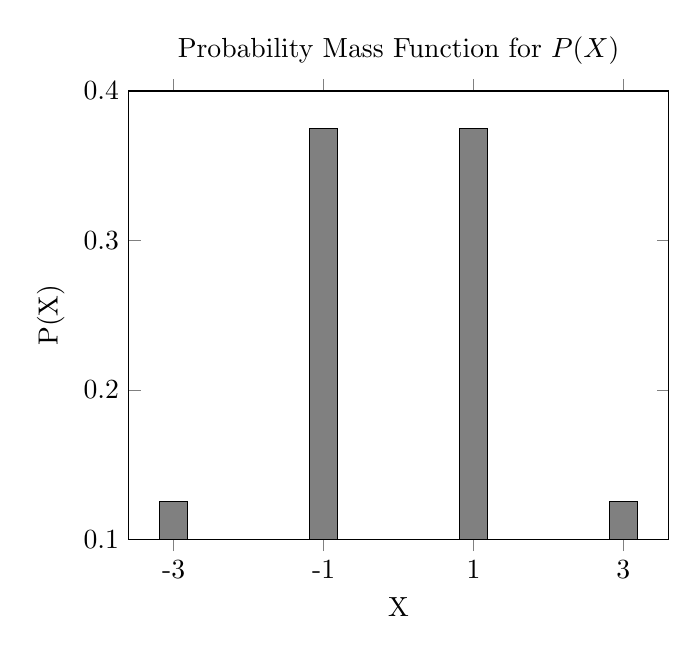
\begin{tikzpicture}
        \begin{axis}[
                title = {Probability Mass Function for $P(X)$},
                xlabel = {X},
                ylabel = {P(X)},
                symbolic x coords={-3,-2,-1,0,1,2,3},
                xtick=data,
                ybar,
            ]
            \addplot[fill=gray] coordinates {
                (-3, 0.125)
                (-1, 0.375)
    		    (1, 0.375)
    		    (3, 0.125)
    	    };
        \end{axis}
    \end{tikzpicture}
\end{center}

\indent The cumulative probabilities are as follows:

\begin{center}
    \begin{tabular}{c|c} 
        $X$ & $CDF(X)$ \\
        \hline
        $-3$ & $0.125$ \\ 
        $-1$ & $0.5$ \\ 
        $1$ & $0.875$ \\ 
        $3$ & $1.0$
    \end{tabular}
\end{center}

\indent They can be graphed like so:

\begin{center}
    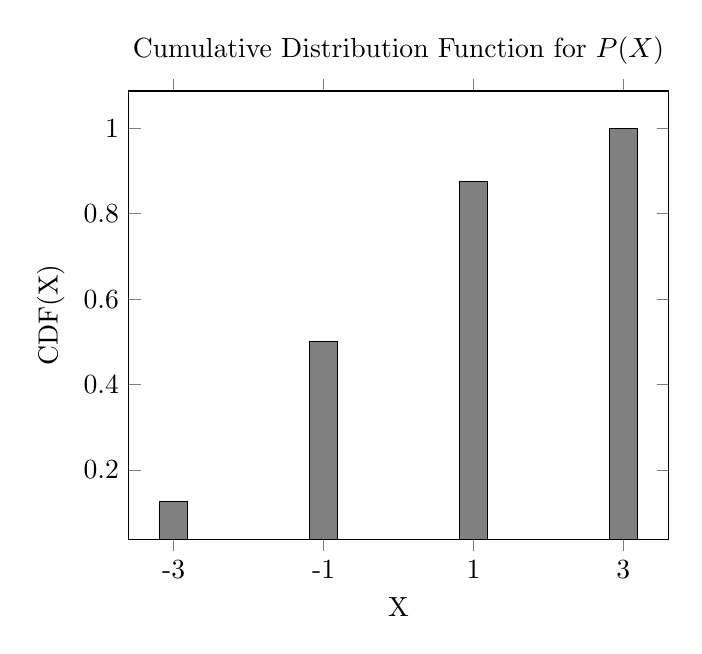
\begin{tikzpicture}
        \begin{axis}[
                title = {Cumulative Distribution Function for $P(X)$},
                xlabel = {X},
                ylabel = {CDF(X)},
                symbolic x coords={-3,-2,-1,0,1,2,3},
                xtick=data,
                ybar,
            ]
            \addplot[fill=gray] coordinates {
                (-3, 0.125)
                (-1, 0.5)
    		    (1, 0.875)
    		    (3, 1.0)
    	    };
        \end{axis}
    \end{tikzpicture}
\end{center}

\section*{Question 3}

\noindent (a) It's not possible for any die roll to be less than $1$.

$$ P(X \geq 1) = 1.0 $$

\noindent (b) The probability that every die rolls is greater than or equal to $2$ is the probability that none of the dice rolls are $1$. Thus, for each roll there are $5$ valid results.

$$ P(X \geq 2) = \left( \frac{5}{6} \right)^4 = 0.48225 $$

\noindent (c) The probability that $P(X \leq 1)$ is the inverse of the probability that none of the dice rolls are $1$.

$$ P(X \leq 1) = 1 - \left( \frac{5}{6} \right)^4 = 0.51774 $$

\indent The probability that $P(X \leq 2)$ is the inverse of the probability that none of the dice rolls are $1$ or $2$ - this is the cumulative probability of $P(X \leq 1) + P(X \leq 2)$.

$$ P(X \leq 2) = 1 - \left( \frac{4}{6} \right)^4 = 0.80246 $$

\indent There is an obvious formula here:

$$ P(X \leq k) = 1 - \left( \frac{6 - k}{6} \right)^4, 1 \leq k \leq 6 $$

\indent Replacing $k$ with the remaining values from $3$ to $6$ gives us the following probabilities:

$$ P(X \leq 3) = 1 - \left( \frac{3}{6} \right)^4 = 0.9375 $$
$$ P(X \leq 4) = 1 - \left( \frac{2}{6} \right)^4 = 0.98765 $$
$$ P(X \leq 5) = 1 - \left( \frac{1}{6} \right)^4 = 0.99922 $$
$$ P(X \leq 6) = 1 - \left( \frac{0}{6} \right)^4 = 1.0 $$

\indent This can be graphed like so:

\begin{center}
    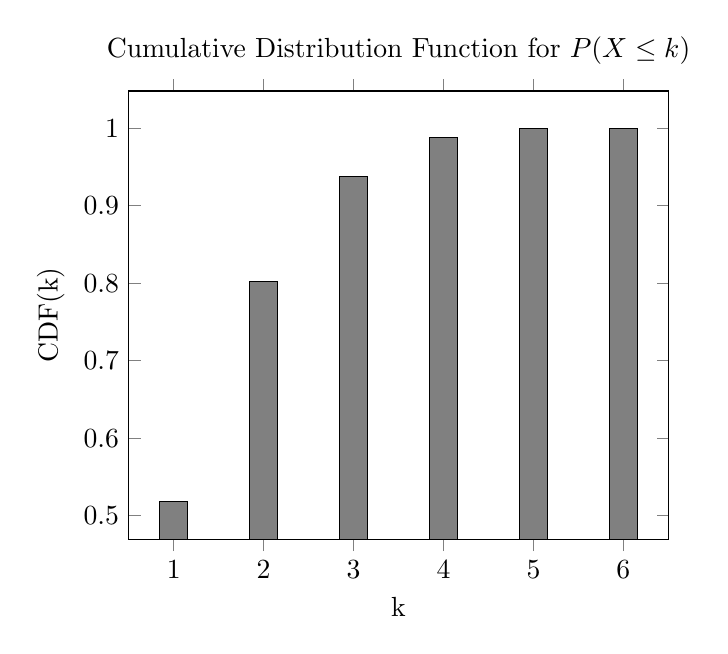
\begin{tikzpicture}
        \begin{axis}[
                title = {Cumulative Distribution Function for $P(X \leq k)$},
                xlabel = {k},
                ylabel = {CDF(k)},
                symbolic x coords={1,2,3,4,5,6},
                xtick=data,
                ybar,
            ]
            \addplot[fill=gray] coordinates {
                (1, 0.51774)
                (2, 0.80246)
    		    (3, 0.9375)
    		    (4, 0.98765)
    		    (5, 0.99922)
    		    (6, 1.0)
    	    };
        \end{axis}
    \end{tikzpicture}
\end{center}

\end{document}
